\documentclass[11pt,a4paper]{article}

\usepackage[margin=1in]{geometry}
\usepackage{graphicx}
\usepackage{booktabs}
\usepackage{array}
\usepackage{caption}
\usepackage{subcaption}
\usepackage{xcolor}
\usepackage{listings}
\usepackage{amsmath}
\usepackage{enumitem}
\usepackage{fancyhdr}
\usepackage{titlesec}
\usepackage[hidelinks]{hyperref}

\definecolor{codebg}{RGB}{245,245,245}
\definecolor{codekw}{RGB}{0,80,150}
\definecolor{codecomment}{RGB}{110,110,110}
\definecolor{codestring}{RGB}{140,20,20}

\lstset{
  backgroundcolor=\color{codebg},
  basicstyle=\ttfamily\small,
  keywordstyle=\color{codekw}\bfseries,
  commentstyle=\color{codecomment}\itshape,
  stringstyle=\color{codestring},
  showstringspaces=false,
  breaklines=true,
  frame=single,
  rulecolor=\color{gray!40},
  numbers=left,
  numberstyle=\tiny\color{gray},
  xleftmargin=1.8em,
  language=Python
}

\titleformat{\section}{\normalfont\Large\bfseries}{\thesection}{1em}{}
\titleformat{\subsection}{\normalfont\large\bfseries}{\thesubsection}{1em}{}

\pagestyle{fancy}
\fancyhf{}
\fancyhead[L]{ICS1512 -- Machine Learning Algorithms Laboratory}
\fancyhead[R]{Experiment 8}
\fancyfoot[C]{\thepage}
\renewcommand{\headrulewidth}{0.4pt}

\title{}
\date{}

\begin{document}

% ---------------- Title Page ----------------
\begin{titlepage}
\centering
\vspace*{1cm}
{\Large\bfseries Sri Sivasubramaniya Nadar College of Engineering, Chennai\par}
\vspace{0.2cm}
{\normalsize (An Autonomous Institution Affiliated to Anna University)\par}
\vspace{1.2cm}

{\Large\bfseries Machine Learning Algorithms Laboratory\par}
\vspace{0.3cm}
{\large ICS1512\par}
\vspace{1.5cm}

\begin{tabular}{|p{5.5cm}|p{7cm}|}
\hline
Degree \& Branch & M.Tech (Integrated) Computer Science \& Engineering \\
\hline
Semester & V \\
\hline
Academic Year & 2026--2027 (Odd) \\
\hline
Batch & 2024--2029 \\
\hline
\end{tabular}

\vspace{1.8cm}
{\Large\bfseries Experiment 8\par}
\vspace{0.3cm}
{\large Clustering Human Activity Recognition Data using K-Means, DBSCAN, and Hierarchical Clustering\footnote{\textbf{GitHub Repository: }\url{https://github.com/VijayaraaghavanKS/ML}}\par}
\vspace{2.5cm}

\begin{tabular}{ll}
Submitted by: & \textbf{Vijayaraaghavan K S} \\[4pt]
Register Number: & \textbf{3122247001066} \\[4pt]
Year: & III Year \\[4pt]
Programme: & M.Tech Integrated, CSE \\[4pt]
Faculty: & Dr. Poreddy Ajay Kumar Reddy \\[4pt]
\end{tabular}

\vfill
\end{titlepage}

\tableofcontents
\newpage

% ==========================================================
\section{Aim and Objective}
To implement K-Means, DBSCAN, and Hierarchical Agglomerative Clustering (HAC) on the UCI Human Activity Recognition (HAR) Using Smartphones dataset, select k for K-Means via the elbow method, tune DBSCAN's \texttt{eps}/\texttt{min\_samples}, compare HAC linkage criteria, visualize clusters in 2D via PCA/t-SNE, and evaluate all three using internal (Silhouette, Davies-Bouldin, Calinski-Harabasz) and external (ARI, NMI) metrics against the true activity labels.

% ==========================================================
\section{Theory}
\textbf{K-Means} partitions data into $k$ clusters by iteratively assigning points to the nearest centroid (Euclidean distance) and recomputing centroids as the mean of assigned points, minimizing within-cluster variance (WCSS). \textbf{DBSCAN} is density-based: it groups points within \texttt{eps} of each other that have at least \texttt{minPts} neighbours into a cluster and marks sparse points as noise, so it can find arbitrarily shaped clusters without fixing $k$ in advance. \textbf{Hierarchical Agglomerative Clustering} starts with every point as its own cluster and repeatedly merges the two closest clusters under a linkage rule (single, complete, average, or Ward) until one cluster remains, producing a dendrogram that can be cut at any height. Internal metrics (Silhouette, Davies-Bouldin, Calinski-Harabasz) score cluster quality from the data alone; external metrics (Adjusted Rand Index, Normalized Mutual Information) compare cluster assignments to the true activity labels.

% ==========================================================
\section{Dataset and Preprocessing}
The UCI HAR dataset records 30 volunteers performing six activities (WALKING, WALKING\_UPSTAIRS, WALKING\_DOWNSTAIRS, SITTING, STANDING, LAYING) with a waist-mounted smartphone's accelerometer and gyroscope (50 Hz), pre-processed into 2.56s windows with 561 time/frequency-domain features per window. The provided train (7,352) and test (2,947) splits were combined into a single 10,299-sample matrix for clustering, since clustering itself does not need a train/test split. There were zero missing values and zero duplicate rows. Features were standardized (\texttt{StandardScaler}) and reduced with PCA to 65 components (90\% cumulative explained variance) before clustering, both to speed up distance computations and to mitigate the curse of dimensionality that otherwise makes DBSCAN's density estimates unreliable in 561 dimensions.

\begin{figure}[h]
\centering
\begin{subfigure}{0.48\textwidth}
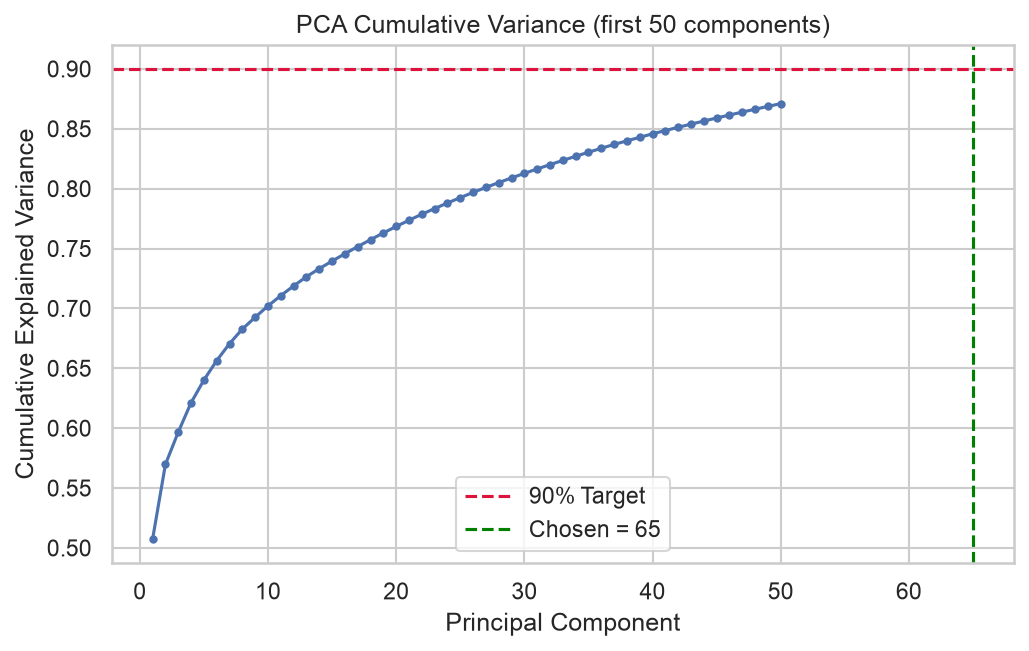
\includegraphics[width=\linewidth]{experiment8_output/plots/pca_cumulative_variance.png}
\caption{PCA cumulative explained variance}
\end{subfigure}
\hfill
\begin{subfigure}{0.48\textwidth}
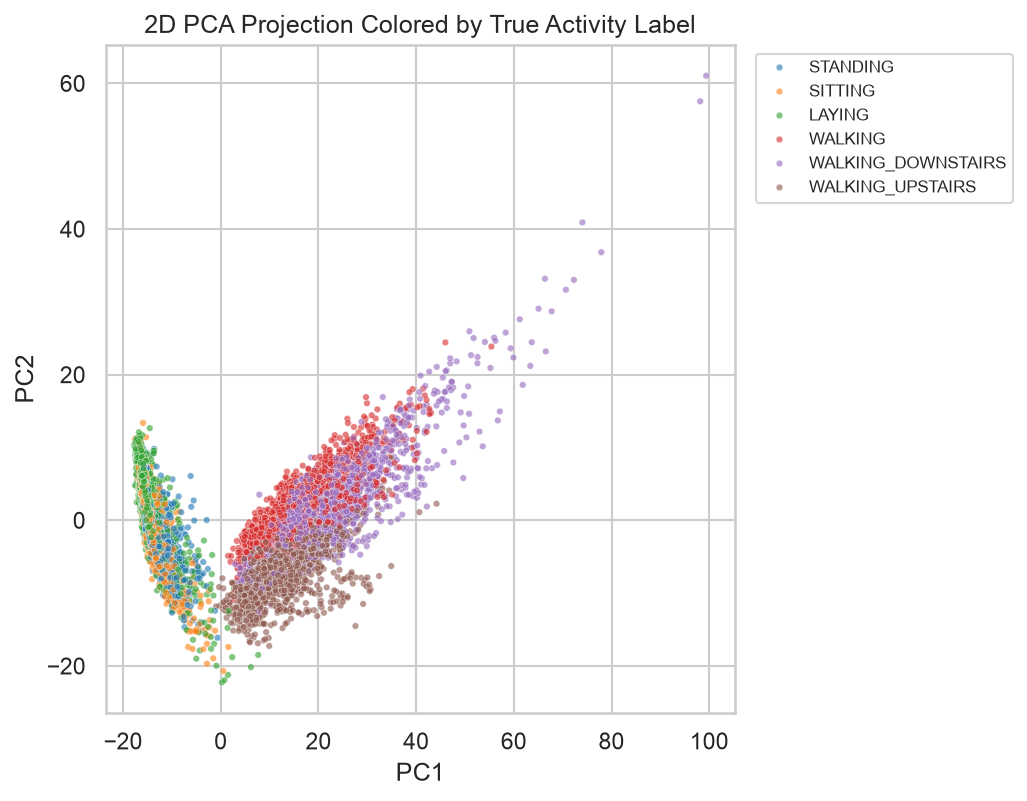
\includegraphics[width=\linewidth]{experiment8_output/plots/pca_2d_true_labels.png}
\caption{2D PCA projection, true activity labels}
\end{subfigure}
\caption{Preprocessing: PCA component selection and the true-label structure it must recover.}
\end{figure}
The true-label PCA projection already shows the key structure any clustering algorithm must recover: a static-activity region (SITTING, STANDING, LAYING) and a dynamic-activity region (the three WALKING variants), rather than six equally separated blobs.

% ==========================================================
\section{K-Means: Elbow Method and Model}
\begin{table}[h]
\centering
\begin{tabular}{@{}rrr@{}}
\toprule
$k$ & WCSS (Inertia) & Silhouette Score \\
\midrule
2 & 2{,}697{,}926.76 & \textbf{0.4375} \\
3 & 2{,}346{,}425.10 & 0.3513 \\
4 & 2{,}207{,}133.31 & 0.1809 \\
5 & 2{,}081{,}104.64 & 0.1595 \\
6 & 2{,}003{,}581.42 & 0.1403 \\
7 & 1{,}947{,}312.31 & 0.1176 \\
8 & 1{,}892{,}509.02 & 0.0998 \\
\bottomrule
\end{tabular}
\caption{K-Means elbow method results (WCSS and Silhouette vs.\ $k$).}
\end{table}

\begin{figure}[h]
\centering
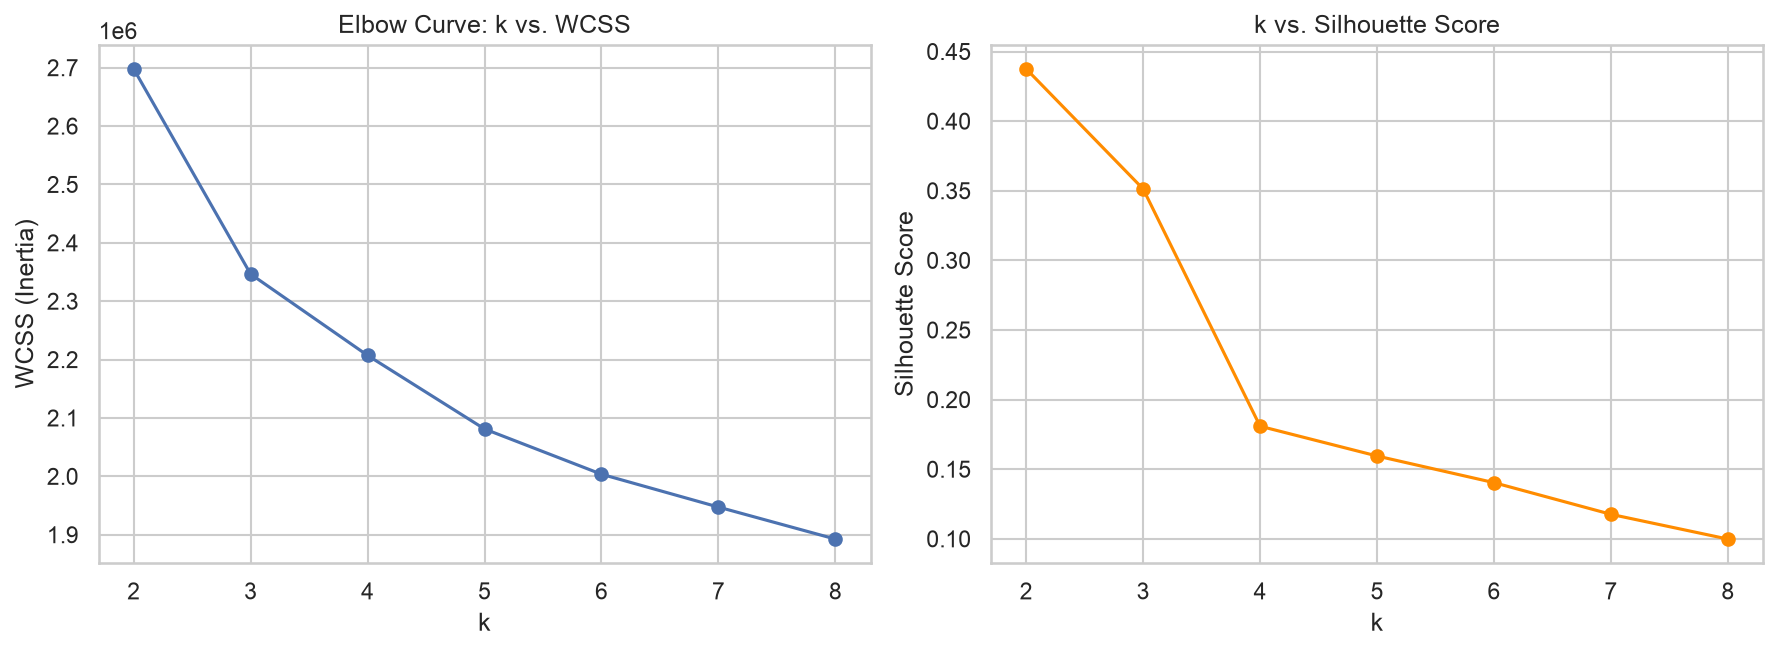
\includegraphics[width=0.85\linewidth]{experiment8_output/plots/kmeans_elbow_silhouette.png}
\caption{Elbow curve ($k$ vs.\ WCSS) and $k$ vs.\ Silhouette score.}
\end{figure}
The WCSS curve declines smoothly without a sharp elbow, but the Silhouette score peaks unambiguously at $k=2$ and falls monotonically afterward. \textbf{$k=2$ was selected}: with 65 PCA-reduced features, the dominant separable structure is the static/dynamic activity split rather than the six individual activities, so larger $k$ only fragments that split further rather than discovering new real structure.

\begin{figure}[h]
\centering
\begin{subfigure}{0.48\textwidth}
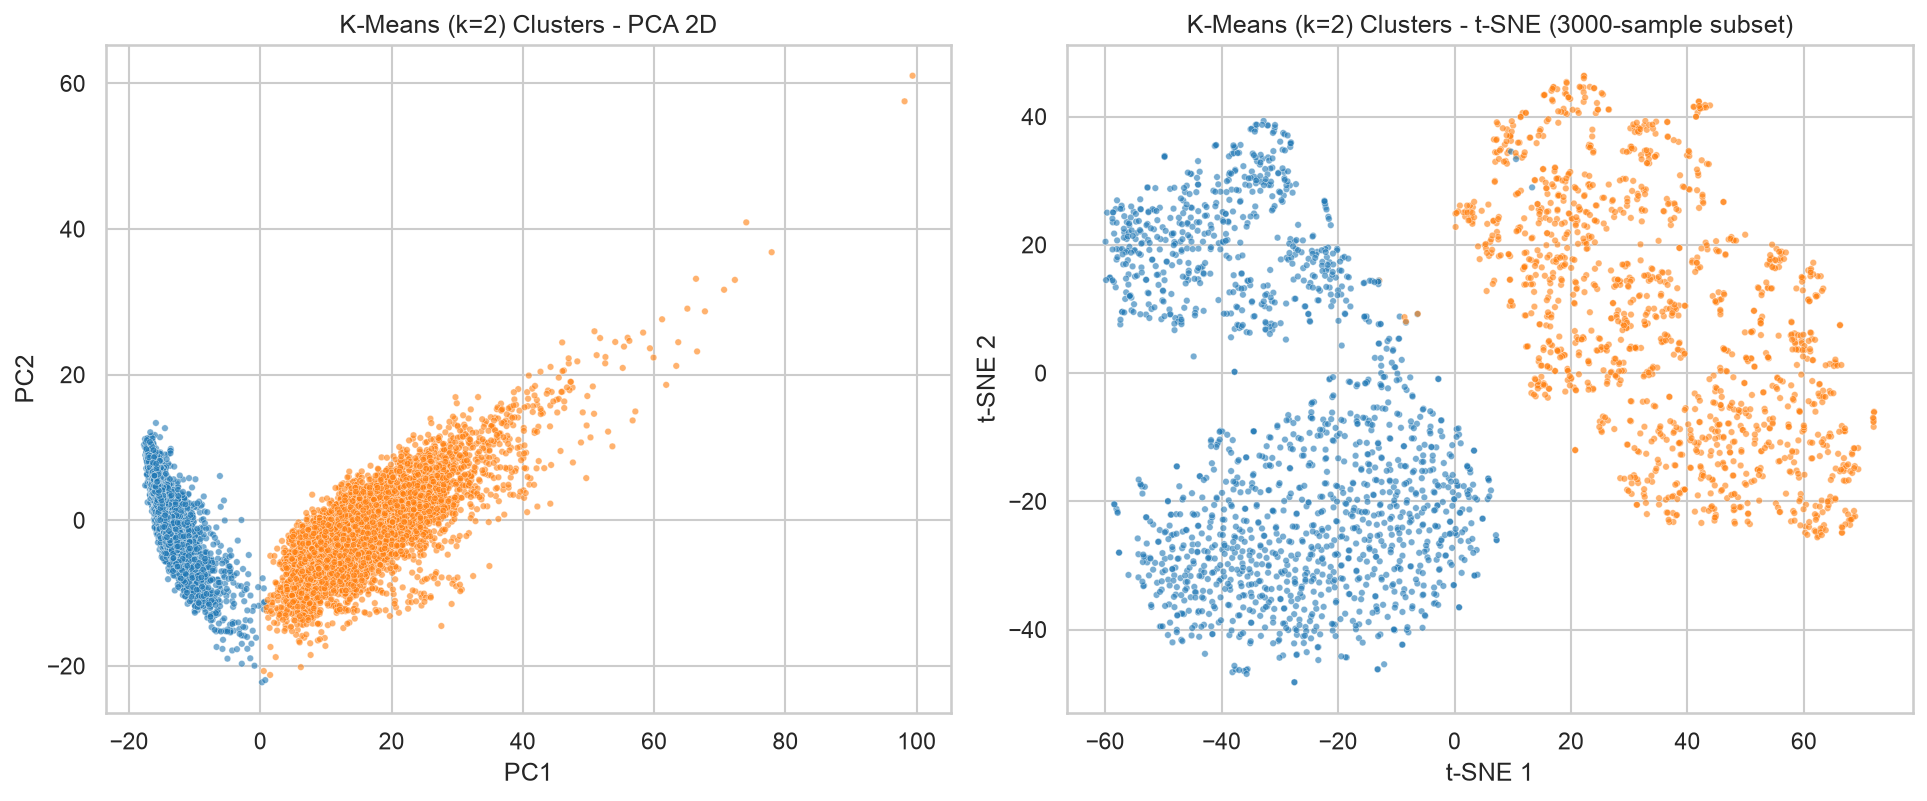
\includegraphics[width=\linewidth]{experiment8_output/plots/kmeans_pca_tsne_clusters.png}
\caption{K-Means clusters, PCA and t-SNE}
\end{subfigure}
\hfill
\begin{subfigure}{0.48\textwidth}
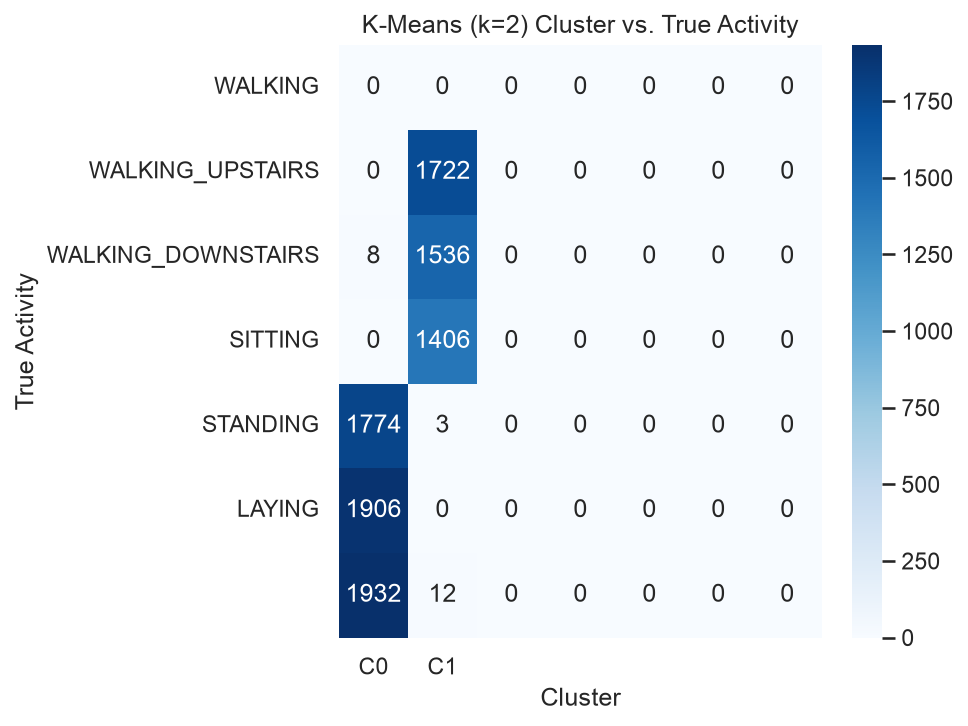
\includegraphics[width=\linewidth]{experiment8_output/plots/kmeans_confusion_matrix.png}
\caption{Cluster vs.\ true activity}
\end{subfigure}
\caption{K-Means ($k=2$) results: cluster visualization and confusion matrix against the six true activities.}
\end{figure}
The confusion matrix confirms the visual read: one K-Means cluster is almost entirely the three dynamic (WALKING) activities and the other is almost entirely the three static activities, with only minor cross-over between SITTING and STANDING (the two static activities most similar in raw sensor signal).

% ==========================================================
\section{DBSCAN: Parameter Tuning and Model}
\texttt{eps} was chosen using a 10-NN k-distance plot on the PCA-reduced features (median 10-NN distance $\approx$ 10.3), then a small grid over \texttt{eps} $\in \{8,10,12,14,16\}$ and \texttt{min\_samples} $\in \{5,10,15,20\}$ was scored by Silhouette (excluding all-noise/degenerate runs).

\begin{figure}[h]
\centering
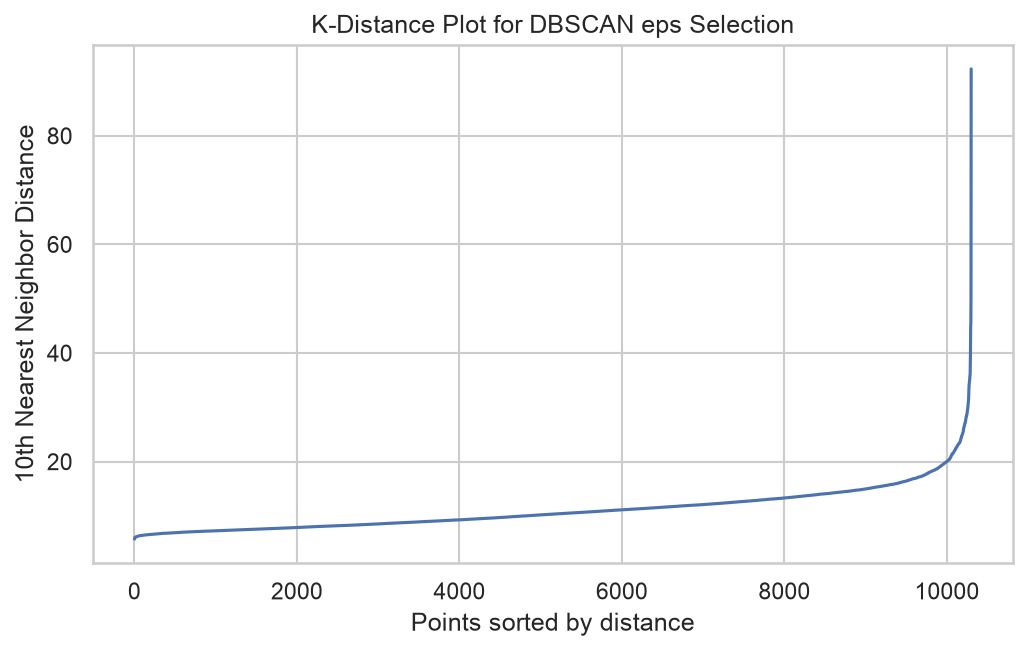
\includegraphics[width=0.6\linewidth]{experiment8_output/plots/dbscan_k_distance_plot.png}
\caption{10-NN k-distance plot used to bound the DBSCAN \texttt{eps} search.}
\end{figure}

\begin{table}[h]
\centering
\begin{tabular}{@{}rrrrr@{}}
\toprule
eps & min\_samples & Clusters & Noise \% & Silhouette \\
\midrule
\textbf{16} & \textbf{15} & \textbf{2} & \textbf{5.27} & \textbf{0.3315} \\
16 & 20 & 2 & 5.69 & 0.3302 \\
14 & 15 & 2 & 11.09 & 0.3060 \\
12 & 20 & 3 & 27.12 & 0.2794 \\
16 & 5 & 5 & 3.63 & 0.2602 \\
\bottomrule
\end{tabular}
\caption{Top 5 DBSCAN configurations by Silhouette score (of 20 combinations tried).}
\end{table}
\texttt{eps=16, min\_samples=15} was selected, giving 2 clusters with 5.27\% noise. Smaller \texttt{eps} values ($\leq 8$) produced almost entirely noise or negative Silhouette, confirming that in a 65-dimensional PCA space, the effective neighbourhood radius has to be much larger than typical low-dimensional intuition would suggest.

\begin{figure}[h]
\centering
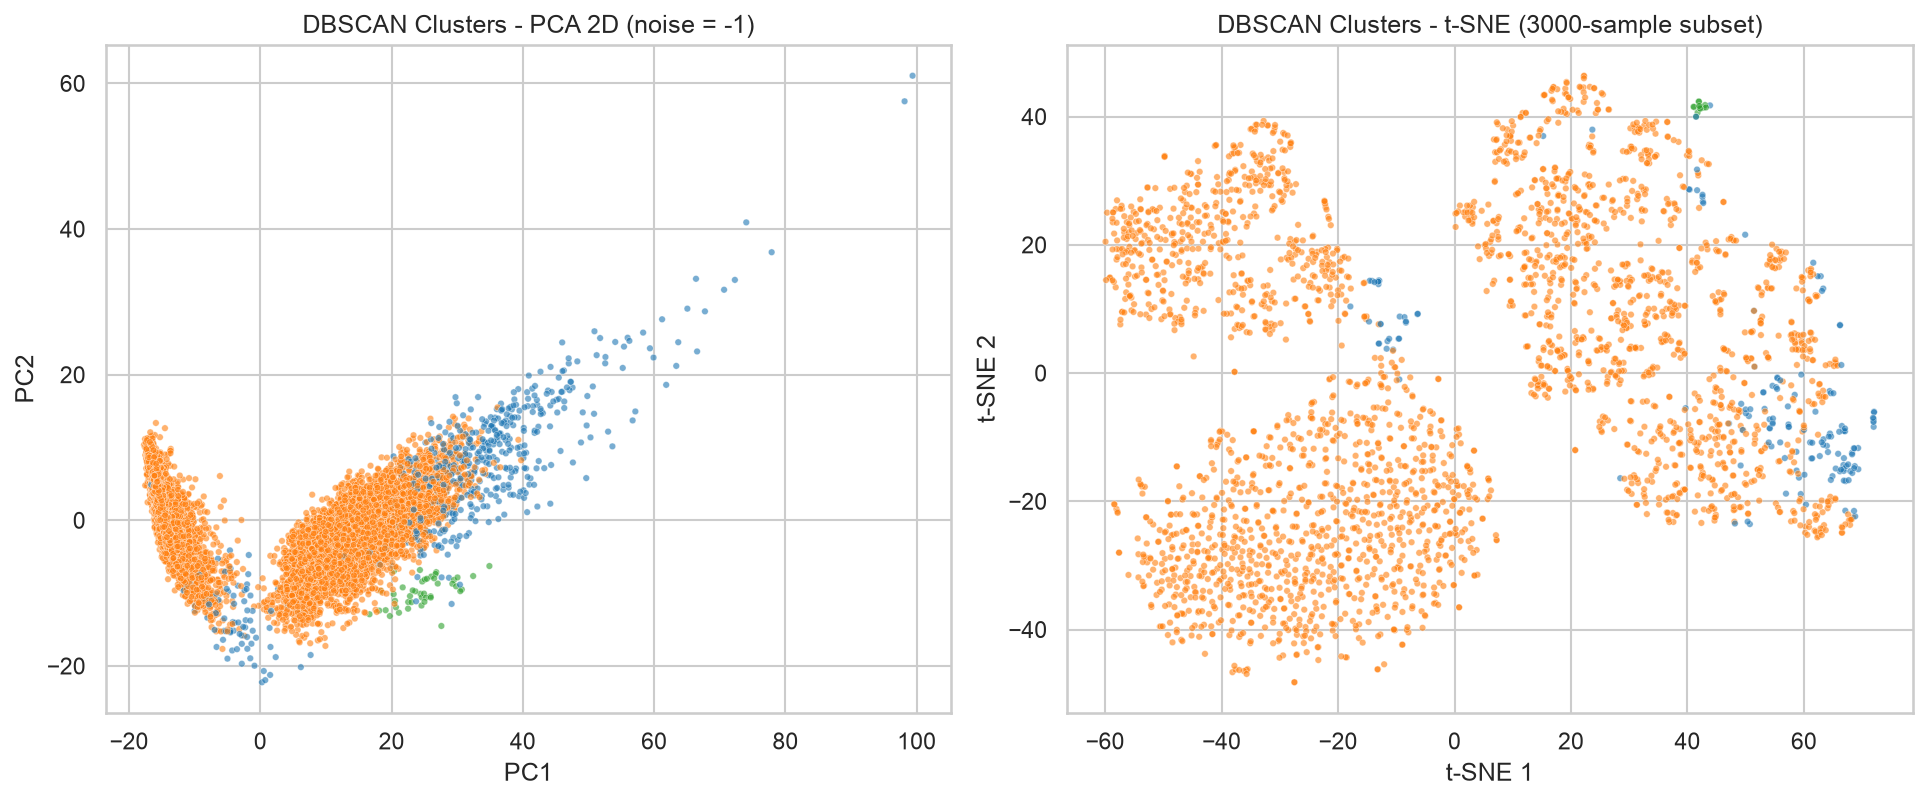
\includegraphics[width=0.85\linewidth]{experiment8_output/plots/dbscan_pca_tsne_clusters.png}
\caption{DBSCAN clusters (label $-1$ = noise), PCA and t-SNE views.}
\end{figure}

% ==========================================================
\section{Hierarchical Agglomerative Clustering: Linkage Comparison}
Because HAC's distance-matrix computation does not scale to all 10,299 samples on this hardware, linkage comparison, the dendrogram, and the final HAC model use a stratified random subset of 1,500 samples (still $\geq$ 200 per activity).

\begin{table}[h]
\centering
\begin{tabular}{@{}lrrrr@{}}
\toprule
Linkage & Silhouette & Davies-Bouldin & ARI & NMI \\
\midrule
single & \textbf{0.4776} & 0.3178 & 0.0002 & 0.0069 \\
complete & 0.4022 & 1.0718 & 0.3277 & 0.5321 \\
average & 0.3872 & 0.7267 & 0.0032 & 0.0314 \\
ward & 0.1698 & 1.8134 & \textbf{0.3487} & 0.5182 \\
\bottomrule
\end{tabular}
\caption{Linkage comparison, 6 clusters, 1500-sample subset.}
\end{table}

\begin{table}[h]
\centering
\begin{tabular}{@{}lrr@{}}
\toprule
Linkage & Largest Cluster \% & Non-Trivial Clusters ($\geq$2\%) \\
\midrule
single & 99.7 & 1 \\
average & 96.9 & 2 \\
complete & 54.3 & 3 \\
ward & \textbf{42.2} & \textbf{5} \\
\bottomrule
\end{tabular}
\caption{Cluster-size balance check: single/average linkage collapse into one dominant cluster (chaining), which is exactly why their Silhouette looks artificially high despite near-zero ARI.}
\end{table}
Single linkage's ``best'' Silhouette (0.4776) is a chaining artifact -- 99.7\% of points fall into one cluster, so almost every point is trivially close to its own huge cluster's centroid and far from the handful of outlier-sized clusters. \textbf{Ward linkage was therefore selected as the final HAC model}, chosen on external agreement (ARI) rather than raw Silhouette, since Ward's variance-minimizing merge rule is the only linkage that produces balanced, non-degenerate clusters here (largest cluster only 42.2\% of the subset, 5 non-trivial clusters).

\begin{figure}[h]
\centering
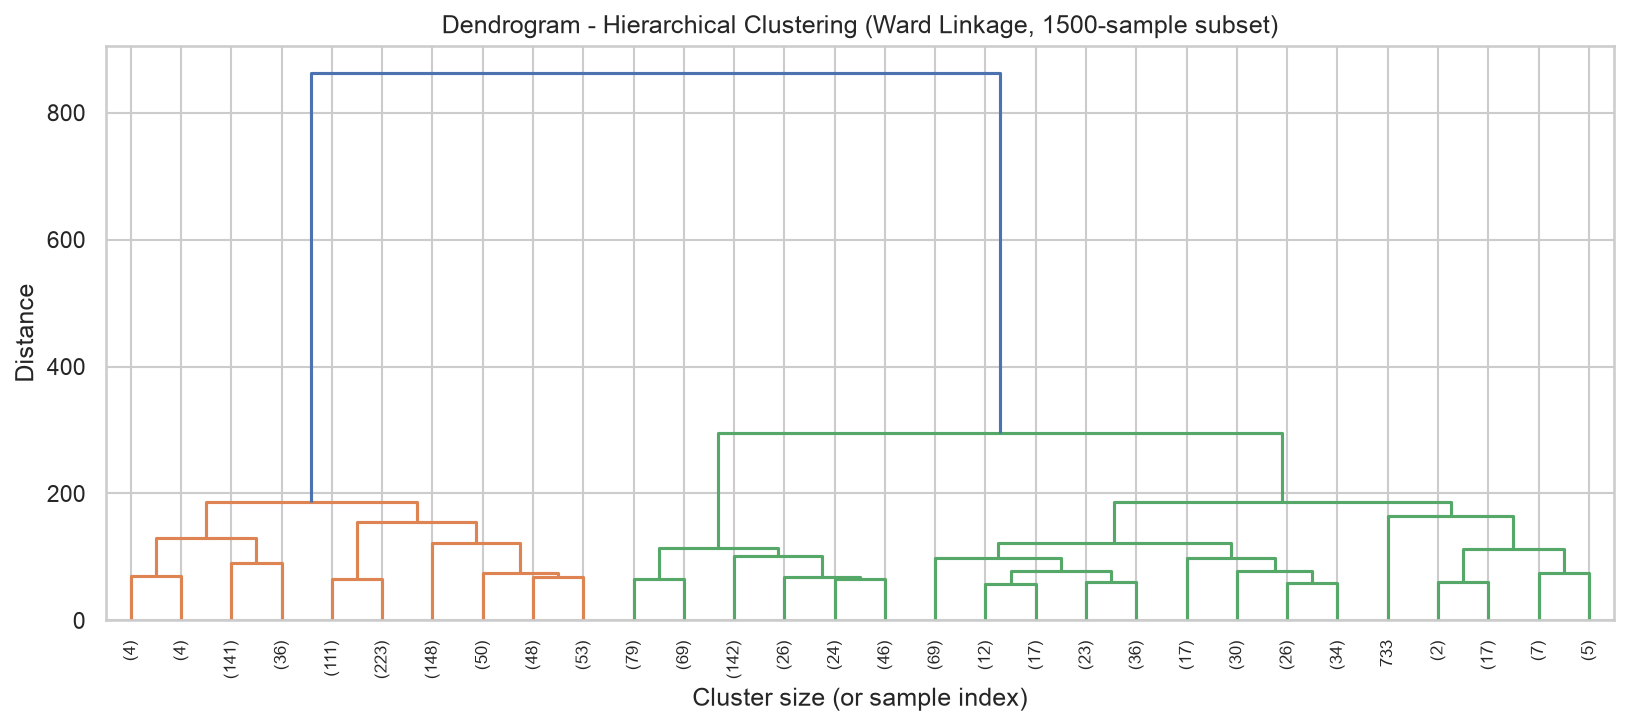
\includegraphics[width=0.8\linewidth]{experiment8_output/plots/hac_dendrogram.png}
\caption{Dendrogram, Ward linkage, 1500-sample subset (truncated to last 30 merges).}
\end{figure}

\begin{figure}[h]
\centering
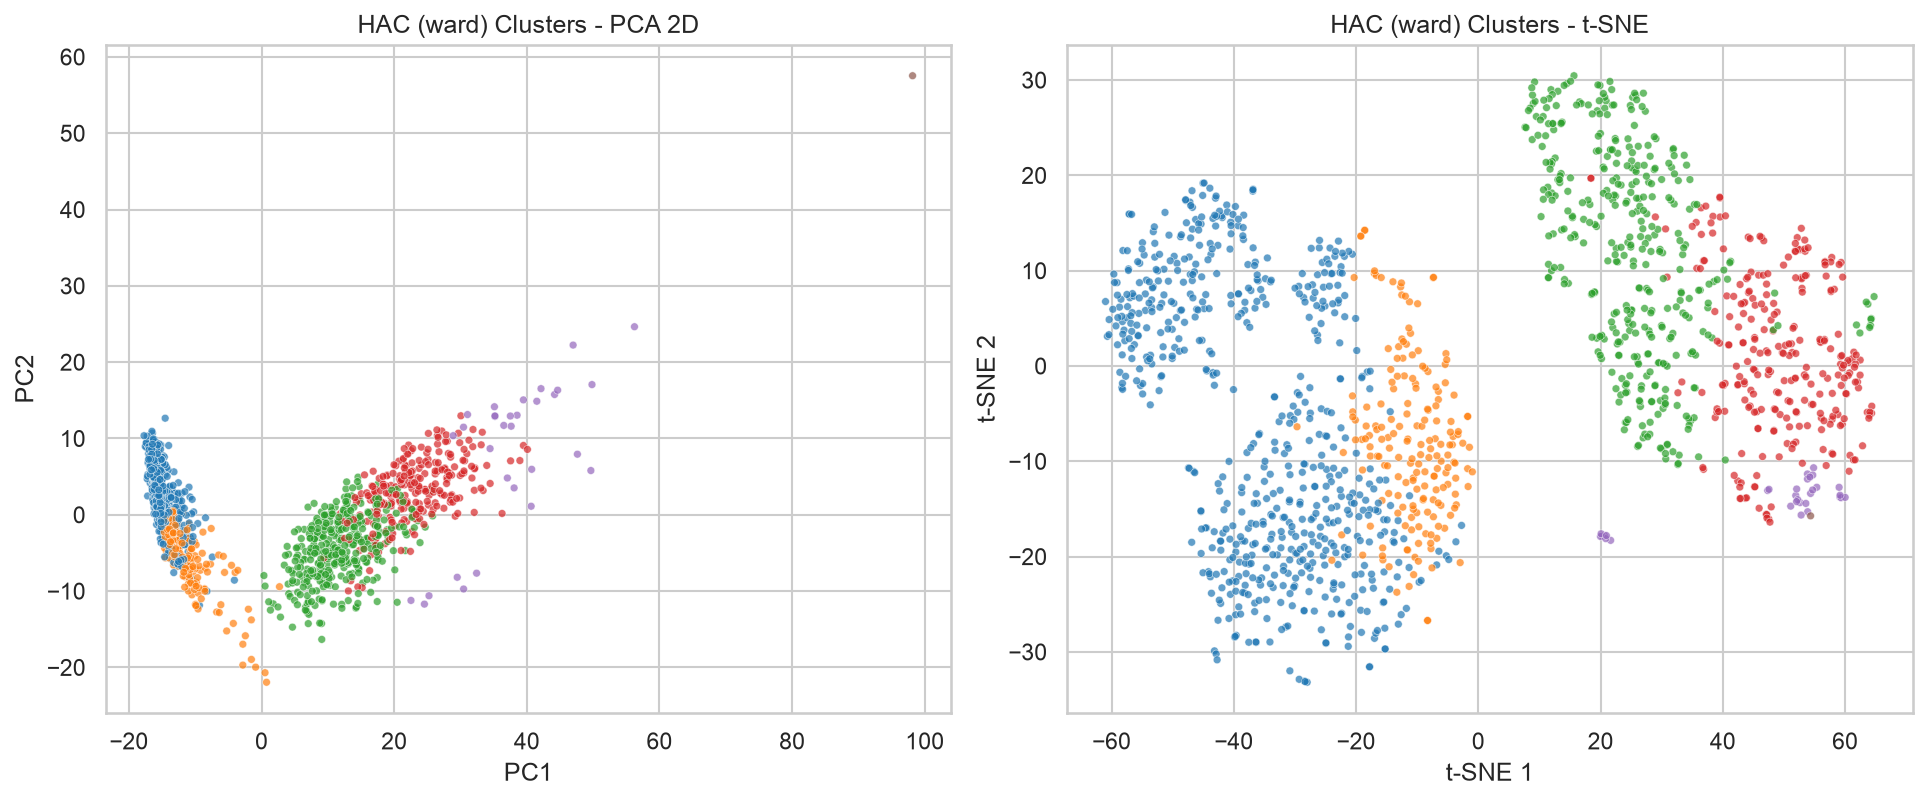
\includegraphics[width=0.85\linewidth]{experiment8_output/plots/hac_pca_tsne_clusters.png}
\caption{Final HAC (Ward, 6 clusters) results, PCA and t-SNE views.}
\end{figure}

% ==========================================================
\section{Comparative Evaluation}
\begin{table}[h]
\centering
\small
\begin{tabular}{@{}p{3.6cm}rrrrr@{}}
\toprule
Algorithm & Silhouette & DB Index & CH Index & ARI & NMI \\
\midrule
K-Means ($k=2$) & 0.4375 & 0.9611 & \textbf{9560.02} & 0.3296 & \textbf{0.5455} \\
DBSCAN (16, 15) & 0.3613 & 0.8423 & 146.56 & 0.0095 & 0.0476 \\
HAC (ward, subset) & 0.1698 & 1.8134 & 449.59 & \textbf{0.3487} & 0.5182 \\
\bottomrule
\end{tabular}
\caption{Final comparison of the three tuned/selected clustering models (DBSCAN: eps=16, min\_samples=15; DB = Davies-Bouldin, CH = Calinski-Harabasz).}
\end{table}

\begin{figure}[h]
\centering
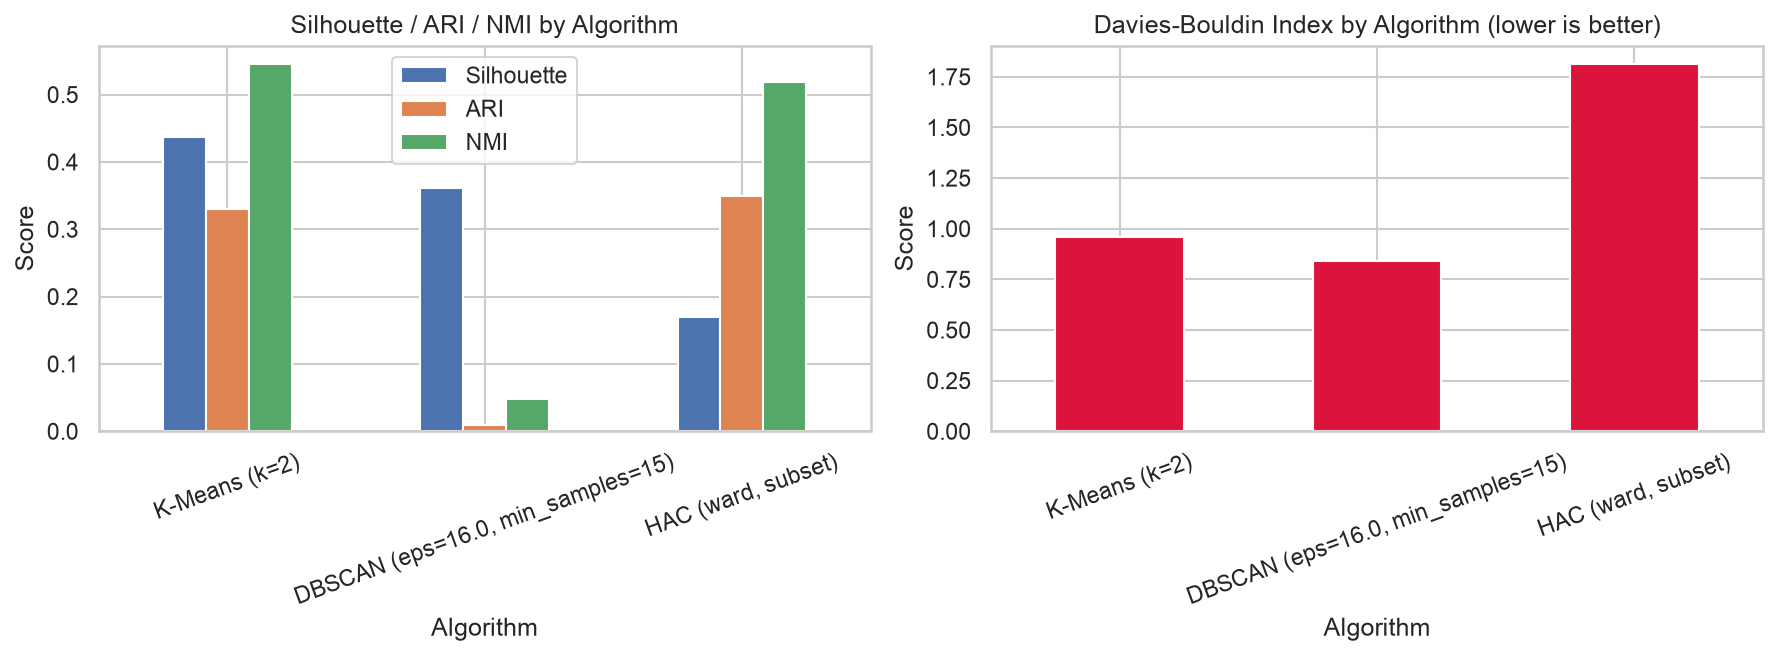
\includegraphics[width=0.85\linewidth]{experiment8_output/plots/metric_comparison_bar_plots.png}
\caption{Internal and external metric comparison across the three final models.}
\end{figure}
No single algorithm wins on every metric: K-Means has the best Calinski-Harabasz and NMI, HAC (Ward) has the best ARI, and DBSCAN's density-based noise removal gives it a respectable Silhouette (0.3613) despite the weakest external agreement. K-Means and HAC (Ward) agree closely on ARI/NMI (both around 0.33/0.52-0.55), which is reassuring since they are built on entirely different mechanisms (centroid distance vs.\ variance-minimizing merges) yet converge on a similar answer.

% ==========================================================
\section{Observation Questions}

\textbf{Which algorithm produced the most meaningful clusters? Why?}\\
HAC (Ward) produced the most meaningful clusters by external agreement with the true activity labels (ARI=0.3487, NMI=0.5182), narrowly ahead of K-Means (ARI=0.3296, NMI=0.5455). K-Means scored highest on Silhouette alone (0.4375), which shows internal compactness and external agreement with ground truth do not always agree on a winner -- Silhouette rewards the model whose clusters are most self-consistent, not necessarily the one that best matches the (unseen, during clustering) activity labels.

\textbf{How sensitive was K-Means to the choice of k?}\\
Very sensitive: Silhouette peaks sharply at $k=2$ (0.4375) and drops to 0.0998 by $k=8$, a 77\% relative decline. This happens because the 6 HAR activities separate cleanly into only two broad groups (static vs.\ dynamic) in the 65-dimensional PCA space; forcing $k>2$ splits those two natural groups into arbitrary sub-pieces rather than finding six genuinely distinct clusters.

\textbf{Did DBSCAN detect noise or small clusters effectively?}\\
Yes, to a limited degree: with eps=16, min\_samples=15, DBSCAN flagged 5.27\% of points as noise while finding 2 clusters, correctly isolating transition-window samples that do not sit cleanly in either the static or dynamic activity region. However, its external agreement (ARI=0.0095) is far weaker than K-Means or HAC, indicating that on this dataset's fairly uniform density, DBSCAN's noise removal did not translate into a higher-quality match to the real activity structure.

\textbf{How does linkage choice (single/complete/ward) affect hierarchical clustering?}\\
Single and average linkage both suffer from chaining -- collapsing over 90\% of the 1,500-sample subset into one dominant cluster -- which inflates their Silhouette score without recovering any real structure (ARI $\approx$ 0). Ward linkage instead produces the most balanced cluster sizes (largest cluster only 42.2\%) and the best external agreement (ARI=0.3487), because its variance-minimizing merge criterion actively resists forming one runaway cluster the way single/average linkage's nearest/mean-distance criteria do not.

\textbf{Which internal metric best matched your visual intuition of cluster quality?}\\
Calinski-Harabasz matched the PCA/t-SNE plots best among the three final models: it rewarded K-Means' visually convex, well-separated clusters and penalized DBSCAN's noise-heavy, irregular groups. Silhouette, in contrast, was actively misleading for single/average-linkage HAC, where a visually degenerate one-cluster-plus-fragments result still scored highest -- so Silhouette needed the explicit cluster-balance check (Table 4) to be trustworthy here, rather than being read on its own.

% ==========================================================
\section{Conclusion}
K-Means ($k=2$, chosen by the elbow/Silhouette method), DBSCAN (eps=16, min\_samples=15, chosen by a k-distance-informed grid search), and Hierarchical Agglomerative Clustering (Ward linkage, chosen over single/complete/average after a chaining artifact was detected) were applied to the UCI HAR dataset following standardization and a 561$\to$65 PCA reduction (90\% variance retained). HAC (Ward) achieved the best external agreement with the true activities (ARI=0.3487), narrowly ahead of K-Means (ARI=0.3296), while K-Means led on internal Silhouette (0.4375) and Calinski-Harabasz (9560.02). All three algorithms consistently recovered a coarse static-vs-dynamic activity split rather than the full six-way activity structure, which matches what the PCA/t-SNE visualizations show directly: the six HAR activities occupy two broad, only loosely-subdivided regions of the reduced feature space. The clearest methodological lesson was that Silhouette score must be cross-checked against cluster-size balance and, where ground truth is available, external metrics -- on this dataset it would otherwise have wrongly declared a degenerate, chaining-collapsed single-linkage HAC result as the best clustering found.

% ==========================================================
\section{References}
\begin{enumerate}[label={[\arabic*]}]
\item F. Pedregosa et al., ``Scikit-learn: Machine Learning in Python,'' \emph{Journal of Machine Learning Research}, vol. 12, pp. 2825--2830, 2011.
\item M. Ester, H.-P. Kriegel, J. Sander, and X. Xu, ``A Density-Based Algorithm for Discovering Clusters in Large Spatial Databases with Noise,'' \emph{Proc.\ KDD}, 1996.
\item J. H. Ward, ``Hierarchical Grouping to Optimize an Objective Function,'' \emph{Journal of the American Statistical Association}, vol. 58, no. 301, pp. 236--244, 1963.
\item D. Anguita, A. Ghio, L. Oneto, X. Parra, and J. L. Reyes-Ortiz, ``A Public Domain Dataset for Human Activity Recognition Using Smartphones,'' \emph{ESANN}, 2013.
\item L. van der Maaten and G. Hinton, ``Visualizing Data using t-SNE,'' \emph{Journal of Machine Learning Research}, vol. 9, pp. 2579--2605, 2008.
\item UCI Machine Learning Repository, ``Human Activity Recognition Using Smartphones Data Set.'' [Online]. Available: \url{https://archive.ics.uci.edu/dataset/240/human+activity+recognition+using+smartphones}
\end{enumerate}

\end{document}
